\pdfinfoomitdate=1
\pdftrailerid{}
\pdfsuppressptexinfo=15
\documentclass[11pt]{article}
\usepackage[T1]{fontenc}
\usepackage{lmodern}
\usepackage[margin=1.05in]{geometry}
\usepackage{amsmath,amssymb,amsthm,mathtools}
\usepackage{microtype}
\usepackage{tikz}
\usetikzlibrary{arrows.meta,positioning}
\usepackage{xcolor}
\definecolor{linkblue}{RGB}{20,69,103}
\usepackage[colorlinks=true,linkcolor=linkblue,citecolor=linkblue,urlcolor=linkblue]{hyperref}
\hypersetup{pdftitle={Optimal-order mixing of the Thorp shuffle},pdfauthor={OpenAI},bookmarksopen=true,bookmarksnumbered=true}
\newtheorem{theorem}{Theorem}[section]
\newtheorem{lemma}[theorem]{Lemma}
\newtheorem{proposition}[theorem]{Proposition}
\theoremstyle{remark}
\newtheorem{remark}[theorem]{Remark}
\numberwithin{equation}{section}
\title{Optimal-order mixing of the Thorp shuffle}
\author{OpenAI}
\date{September 26, 2026}
\begin{document}
\maketitle
\begin{abstract}
We prove that the Thorp shuffle on $2^d$ cards mixes in $\Theta(d)$ complete shuffles. The full permutation law after $1600d$ shuffles converges to uniform in total variation as $d\to\infty$, uniformly over the initial deck, while a support count gives a lower bound of $2d-O(1)$.
\end{abstract}

\section{Introduction}\label{sec:introduction}

A single card can become uniformly distributed long before a shuffled
deck is close to uniform. The Thorp shuffle makes this distinction
particularly clear. Split a deck into two equal halves, pair cards that
occupy corresponding positions, and choose the order of each pair by an
independent fair coin. Interleaving the pairs produces the new deck.
For a deck of size $n=2^d$, every individual card is uniform after $d$
shuffles. The question is how much longer it takes to randomize the
joint order of all $n$ cards.

We prove that a constant multiple of $d$ shuffles suffices. Let $q_d$
denote the law of one complete shuffle as a permutation of the
positions, and let $U_n$ be uniform on the symmetric group $S_n$.
Convolution is the law of composition of independent permutations, and
\[
 \|\mu-\nu\|_{\mathrm{TV}}
 =\frac12\sum_g|\mu(g)-\nu(g)|.
\]
Write $t_{\mathrm{mix}}(d)$ for the least nonnegative integer $t$ at which
$\|q_d^{*t}-U_n\|_{\mathrm{TV}}\le1/4$.

\begin{theorem}[Optimal-order mixing]\label{thm:mixing}
As $d\to\infty$,
\[
 \|q_d^{*(1600d)}-U_n\|_{\mathrm{TV}}\longrightarrow0.
\]
For every integer $t\ge0$,
\[
 \|q_d^{*t}-U_n\|_{\mathrm{TV}}
 \ge 1-\frac{2^{tn/2}}{n!}.
\]
Consequently the mixing time at distance $1/4$ satisfies
\[
 t_{\mathrm{mix}}(d)\ge
 \left\lceil\frac2n\log_2\frac{3n!}{4}\right\rceil
 =2d-O(1),
 \qquad t_{\mathrm{mix}}(d)=\Theta(d).
\]
\end{theorem}

One step in this theorem is one complete physical shuffle. Changing the
initial deck translates the permutation law, so its distance from
uniform is unchanged. The upper bound is asymptotic in $d$; the
constant $1600$ is an explicit choice in the proof, not a proposed
sharp constant. Determining a leading constant or a cutoff remains a
separate question.

The full-law conclusion controls every statistic of the final deck and,
in particular, the joint positions of any deterministic selection of
cards, by contraction of total variation under a map. It also shows
that this shuffle produces an approximately uniform permutation using
$O(n\log n)$ independent fair bits: each of the $O(\log n)$ steps uses
$n/2$ bits. The support bound identifies the same order of randomness
as necessary for this construction.

\subsection{History and related work}

Thorp introduced the model in his 1973 study of the effects of
nonrandom shuffling on Faro \cite[Section~3.1]{thorp}. Its simple
pairwise rule conceals a difficult question about dependence across the
whole deck. For dyadic decks, Morris obtained the first bound
polynomial in $d$, namely $O(d^{44})$, using evolving sets and a
chameleon process that tracks conditional card probabilities
\cite{morris44}. Montenegro and Tetali sharpened this analysis to
$O(d^{29})$ by spectral-profile and evolving-set methods
\cite[Theorems~6.14--6.15]{montenegro-tetali2006}.

A second line of attack used relative entropy. Morris related entropy
decay to pairwise card collisions and obtained $O((\log n)^4)$
shuffles for every even $n$ \cite{morris4}. He then proved $O(d^3)$
for $n=2^d$ by a stronger contraction over a block of $d$ shuffles
\cite{morris3}. Theorem~\ref{thm:mixing} attains the logarithmic order
discussed in Jonasson's notes \cite[Section~5]{jonasson} for dyadic
decks. The corresponding optimal-order question for arbitrary even
deck sizes is not addressed by the cube argument here.

Card marginals have also been studied for their own sake and for
cryptography. Morris, Rogaway and Stegers analyzed the joint images of
ordered input lists in their construction of enciphering schemes on
small domains \cite[Theorem~1]{mrs}. Czumaj and V\"ocking proved that
$O((\log n)^2)$ Thorp shuffles mix any fixed fraction of the cards
strictly below one, using non-Markovian couplings and butterfly-network
estimates \cite{CzumajVocking2014}. Our first stage needs a different,
averaged guarantee: after $200d$ shuffles, the joint positions of a
uniformly sampled list of $7n/8$ labels are close to uniform on average
over the list. The passage from these averaged marginals to the full
law is a separate part of the proof.

The conditional-flow method has several predecessors. In the original
Thorp analysis, Morris used a chameleon process to represent the law of a tagged card
conditional on the set-valued trajectory of a collection containing
that card; the conditional probabilities average across available pairs
and are transported across pairs with only one available position
\cite[Section~4, Lemma~3]{morris44}. Hoang, Morris and Rogaway later
used conditional squared energy and a sequential total-variation
comparison to analyze the swap-or-not shuffle
\cite[Section~3, Theorem~3 and Lemma~4]{hmr2014}. Their uniformly random
keys make the next partner uniform over the underlying group.
Here the directions are prescribed cyclically. The exact identity
retaining only one sweep of noise, together with independence of the
two opposite halves during the intervening updates, provides the needed
contraction.

For the final passage to the group, we use complete reducibility and
Schur orthogonality, together with the tableau description and
hook-length formula for symmetric-group degrees
\cite{etingof,sagan}. The inverse-degree summability needed here is a
special case of a stronger theorem of Liebeck and Shalev
\cite[Theorem~2.6]{liebeck-shalev2004}; we give an elementary proof of
the required case. The final total-variation comparison is the
finite-group Fourier method of Diaconis and Shahshahani
\cite[Section~3, Lemma~14]{DiaconisShahshahani1981}.
The additional step here is to turn bounds on complementary card
marginals into operator bounds for matrix Fourier transforms, using a
common trimming and the span of one vector's orbit under a block
subgroup.

\subsection{Proof overview}

Label positions by binary strings of length $d$, the vertices of a
cube. Undoing a deterministic cyclic rotation turns successive shuffles
into switch layers along successive coordinate directions: the two
positions in one switch differ only in the active bit. A sweep through
all $d$ directions takes $d$ physical shuffles.
Section~\ref{sec:model} gives this change of frame and proves the
support lower bound.

For the upper bound, first choose an ordered list of $7n/8$ labels
uniformly and independently of the shuffle. Expose these cards one at
a time. Conditional on the paths already exposed, the next card has a
probability distribution on the remaining positions. On a switch with
two remaining positions its masses are averaged; on a switch with
only one remaining position its mass follows the route fixed by the
exposed path. Subtracting the uniform distribution on the remaining
positions gives a centered flow.

A full sweep of coordinate averages annihilates every mean-zero
vector. The actual conditional update differs from coordinate averaging
only by noise with conditional mean zero on switches with one available
position.
Consequently the expected squared norm at the present time is an exact
weighted sum of noise contributions from the preceding sweep, as
proved in Section~\ref{sec:flow}. To control those contributions,
Section~\ref{sec:contraction} looks back from the next active direction
through the $d-1$ other directions. These updates act independently
inside the two opposite halves. A flow value in one half is therefore
independent of the availability of its partner in the other half,
conditional on the history at the start of this interval. A random list
leaves a positive fraction of available positions in both halves with
high probability. This yields a scalar energy recurrence and then the
averaged marginal estimate of Proposition~\ref{prop:averaged-marginal}
at time $200d$.

The second stage recovers the dependencies involving the omitted
cards. Partition the labels into eight equal blocks, choosing the
partition so that the eight complementary marginals have small total
error. Each marginal is a distribution on cosets of the subgroup that
permutes its omitted block. Removing a small amount of probability
makes all eight coset densities bounded under one common law.
Restrict an irreducible representation of $S_n$ to the product of these
eight subgroups. Each tensor constituent has at least one factor of
small degree. Even with arbitrary multiplicity, the orbit of a single
vector under the corresponding block subgroup spans a space of
controlled dimension.
Averaging projections onto its translates then bounds each Fourier
operator. Sections~\ref{sec:degrees} and~\ref{sec:lift} supply the degree
estimate and this transfer; Section~\ref{sec:completion} combines eight
independent time intervals of $200d$ shuffles and handles parity to complete the proof.

The companion on random coordinate frames gives an independent
$32800d$ proof \cite[Theorem~1.1]{companion-frames}. The
conditional-information companion obtains bounds uniform over specified
input lists \cite[Theorem~1.1]{companion-conditional}, while the Fourier
companion develops general transfers from complementary coset bounds
\cite[Theorem~1.1]{companion-transfer}. The present proof uses none of
these results: its cyclic-coordinate estimate and eight-block transfer
are proved here.

\section{The model and the support obstruction}\label{sec:model}

Let $d\ge1$ be an integer. Identify the positions with \(V=\mathbb F_2^d\), write $e_1,\ldots,e_d$ for its standard basis, and label each card by its initial position. A permutation maps a label to its current position; composition means \((gh)(x)=g(h(x))\). With
\[
 R(x_1,\ldots,x_d)=(x_2,\ldots,x_d,x_1),
\]
one physical shuffle is \(RS\), where \(S\) independently fixes or swaps each pair \(\{x,x+e_1\}\). Thus its action is
\[
 (x_1,u)\longmapsto (u,x_1+\xi_u),
\]
with independent fair bits \(\xi_u\).

Let $S_1,S_2,\ldots$ be independent copies of $S$. If \(Y_t=RS_tY_{t-1}\) is the physical permutation, started from $Y_0=\mathrm{id}$, and \(X_t=R^{-t}Y_t\), then
\[
 X_{t+1}=Q_tX_t,\qquad
 Q_t=R^{-t}S_{t+1}R^t.
\]
The \(Q_t\) are independent matching switches in the directions
\(i_t=1+(t\bmod d)\), since $R^{-t}e_1=e_{i_t}$. A block whose length is a multiple of \(d\) ends in the physical frame. We analyze this cyclic-coordinate process, writing \(\Pi_t=X_t\).

During one full sweep each coordinate of a given card is refreshed
exactly once by a coin fair conditional on the card's earlier path.
These refreshed bits form a uniform binary string. Restoring the
deterministic rotation preserves uniformity, proving the one-card
assertion in the introduction.

Uniform measure is invariant under every position permutation. Starting from any fixed deck translates the law started at the identity and leaves its total-variation distance from uniform unchanged. Moreover, \(t\) shuffles have at most \(2^{tn/2}\) possible coin strings. Their support \(A\) therefore gives
\[
 \|q_d^{*t}-U_n\|_{\mathrm{TV}}
 \ge q_d^{*t}(A)-U_n(A)
 \ge1-\frac{2^{tn/2}}{n!}.
\]
Distance at most \(1/4\) forces \(2^{tn/2}\ge3n!/4\), proving the rounded lower bound. The inequalities \((n/e)^n\le n!\le n^n\) give its asymptotic form.

For completeness, mixing exists in each fixed dimension. A full coordinate sweep has positive probability of being the identity, and of making any specified single cube-edge transposition. Edge transpositions on the connected cube generate \(S_n\). Every permutation can therefore be obtained in some number of sweeps; identity sweeps pad these representations to one common length. The kernel at that length assigns positive mass to every group element and hence dominates a positive multiple of \(U_n\). Iteration proves convergence. This finite-dimensional observation does not assert the numerical bound \(1600d\) for every \(d\).

\section{A conditional flow with one sweep of memory}\label{sec:flow}

Choose an ordered list \((c_1,\ldots,c_k)\) of distinct labels independently of the shuffle. We will ultimately average over uniform lists, but first fix the list. For $0\le\ell<k\le n$, expose the trajectories of its first \(\ell\) cards, and call the next card the tagged card. Let $\mathcal F_s$ be the sigma-field generated by the list and the exposed paths through time $s$. Let \(B_s\) be the positions not occupied by those \(\ell\) cards, so \(m=|B_s|=n-\ell\) is constant. Define
\[
 p_s(x)=\mathbb P\{\Pi_s(c_{\ell+1})=x\mid\mathcal F_s\},
 \qquad
 w_s(x)=p_s(x)-\frac1m\mathbf1_{B_s}(x).
\]
The vector \(w_s\) is supported on \(B_s\), has total sum zero, and has squared norm at most one. Averaging and transport also underlie Morris's chameleon representation \cite[Section~4, Lemma~3]{morris44}. The next lemma identifies the unexposed coins directly for labeled trajectories.

\begin{samepage}
\begin{lemma}[Path cylinders and conditional flow]\label{lem:path-cylinder}
For every feasible specification of the exposed paths through a time $T$,
the visited time--edge coins are fixed and all other coins remain
independent and fair. On a matching edge with two free positions the
conditional masses are averaged; on an edge with one free position its
mass follows the known free route. These rules also transport the uniform
mass on $B_s$ to that on $B_{s+1}$. For $s\le T$, conditioning on the
full exposed paths gives the same tagged-card law at time $s$ as
conditioning on $\mathcal F_s$.
\end{lemma}
\end{samepage}
\begin{proof}
To verify the cylinder assertion, fix any feasible specification of the exposed paths through a terminal time \(T\). The paths determine the visited time-edge pairs and the coin value at every visited pair. Conversely, prescribing these values forces the specified paths, by induction on time: the next position of an exposed card depends only on the coin of its present edge. If two exposed cards share an edge, feasibility gives the same prescribed coin. The path event is therefore a cylinder in the independent coin array. Conditional on it, unvisited coins remain independent and fair.

It follows that an edge with two free positions averages their tagged-card masses. An edge with one free position transports its mass to the uniquely free output specified by the exposed card's next position. These updates also carry the uniform vector on \(B_s\) to the uniform vector on \(B_{s+1}\). Future prescribed coins involve later time coordinates of the array; they do not alter the earlier free coins. Consequently the law at time \(s\), even if initially defined by conditioning on all exposed paths through \(T\), equals this \(\mathcal F_s\)-measurable forward flow. In particular we may use its adaptedness below. Averaging and transport do not increase squared norm. The initial centered point mass has squared norm $1-1/m\le1$, which proves the stated bound on \(w_s\). Figure~\ref{fig:conditional-flow} depicts the two updates.
\end{proof}

\begin{figure}[tb]
\centering
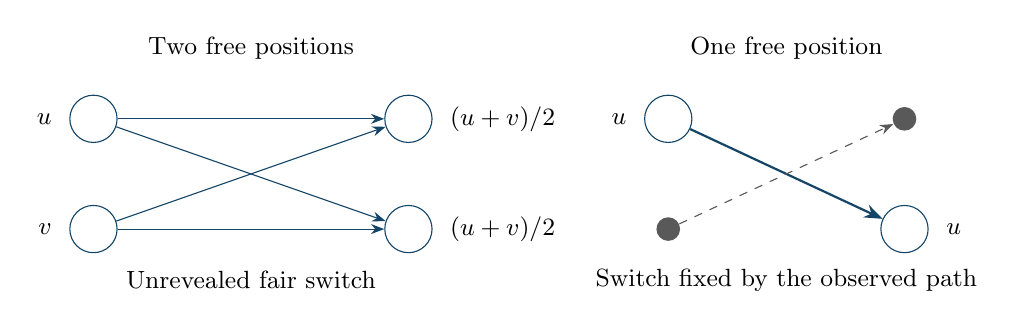
\begin{tikzpicture}[>=Stealth, every node/.style={font=\small},
    free/.style={circle,draw=linkblue,fill=white,minimum size=6mm},
    seen/.style={circle,fill=black!65,minimum size=3mm,inner sep=0pt}]
  \node at (2,2.6) {Two free positions};
  \node[free] (a) at (0,1.7) {};
  \node[free] (b) at (0,0.3) {};
  \node[left=1mm of a] {$u$};
  \node[left=1mm of b] {$v$};
  \node[free] (c) at (4,1.7) {};
  \node[free] (d) at (4,0.3) {};
  \node[right=1mm of c] {$(u+v)/2$};
  \node[right=1mm of d] {$(u+v)/2$};
  \draw[->,linkblue] (a)--(c);
  \draw[->,linkblue] (a)--(d);
  \draw[->,linkblue] (b)--(c);
  \draw[->,linkblue] (b)--(d);
  \node at (2,-0.35) {Unrevealed fair switch};
  \begin{scope}[xshift=7.3cm]
    \node at (1.5,2.6) {One free position};
    \node[free] (e) at (0,1.7) {};
    \node[seen] (f) at (0,0.3) {};
    \node[left=1mm of e] {$u$};
    \node[seen] (g) at (3,1.7) {};
    \node[free] (h) at (3,0.3) {};
    \node[right=1mm of h] {$u$};
    \draw[->,linkblue,thick] (e)--(h);
    \draw[->,black!65,dashed] (f)--(g);
    \node at (1.5,-0.35) {Switch fixed by the observed path};
  \end{scope}
\end{tikzpicture}
\caption{The conditional flow on one matching edge. Open circles are free
positions; filled circles contain an exposed card. A switch with two free
positions averages the centered masses $u,v$. With one free position,
the observed path fixes the switch and transports the centered mass $u$.
The latter case produces the martingale noise before the switch is revealed.}
\label{fig:conditional-flow}
\end{figure}


Let \(A_i\) average a function across every coordinate-\(i\) pair, and write \(x^{(i)}=x+e_i\). Put
\[
 E_s=\mathbb E\|w_s\|_2^2,
 \qquad
 L_s=\sum_x w_s(x)^2\mathbf1_{\{x^{(i_s)}\notin B_s\}},
 \qquad b_s=\mathbb E L_s.
\]
Here the expectation includes the initial list when it is random. Before the next exposed positions are revealed, the transport choices on edges with one free position are independent fair coins. Hence
\begin{equation}\label{eq:h-1}
 w_{s+1}=A_{i_s}w_s+\xi_s,
 \qquad \mathbb E(\xi_s\mid\mathcal F_s)=0.
\end{equation}
On a one-free-position edge whose free endpoint is \(x\), its noise is
\[
 \pm\frac{w_s(x)}2(\delta_x-\delta_{x^{(i_s)}}),
\]
where $\delta_x$ is unit mass at $x$, and the signs are independent on distinct such edges. Other edges contribute no noise.

\begin{lemma}[One-sweep energy identity]\label{lem:energy-memory}
For every \(t\ge d\),
\begin{equation}\label{eq:h-2}
 E_t=\sum_{j=1}^d2^{-j}b_{t-j}.
\end{equation}
\end{lemma}
\begin{proof}
Expand \eqref{eq:h-1} over the last \(d\) layers. The product of all \(d\) coordinate averages maps a vector to its spatial mean, so it annihilates \(w_{t-d}\). Noise terms from distinct times have zero expected cross products: the later term has conditional mean zero and the intervening averages are deterministic. At a fixed time, noises on distinct edges also have zero expected cross products, because their signs are independent conditional on the exposed past. The noise created at time \(t-j\) is followed by averaging in \(j-1\) distinct coordinates other than its own. Its two masses spread over disjoint subcubes, each of size \(2^{j-1}\). The resulting squared norm is \(2^{-j}w_{t-j}(x)^2\). Summing these contributions proves \eqref{eq:h-2}.
\end{proof}

\section{Why the recent noise contracts}\label{sec:contraction}

We bound the recent-noise term \(b_s\) in terms of the energy \(E_s\), then use the resulting decay to control ordered card marginals.

Fix \(s\ge d-1\), put \(a=s-d+1\), and let \(H_0,H_1\) be the two halves defined by coordinate \(i_s\). The updates from \(a\) to \(s\) use every other coordinate once and do not cross these halves. Conditional on \(\mathcal F_a\), the initial free sets \(B_a\cap H_h\) and centered flows \(w_a|_{H_h}\) are fixed, and the future switch arrays in the two halves are independent. The pair \((B_s\cap H_h,w_s|_{H_h})\) is determined by this initial state and the switch array inside \(H_h\).

Every position at time \(a\) in a half is marginally uniform in that half after the intervening \(d-1\) updates: each of its remaining coordinates is refreshed by a conditionally fair coin. Summing this endpoint probability over the free positions at time \(a\) gives, for every \(y\in H_{1-h}\),
\[
 \mathbb P\{y\in B_s\mid\mathcal F_a\}
 =\frac{|B_a\cap H_{1-h}|}{n/2}.
\]
For \(x\in H_h\), the random variables \(w_s(x)^2\) and \(\mathbf1_{\{x^{(i_s)}\in B_s\}}\) depend on opposite future arrays. Their conditional independence therefore yields
\begin{equation}\label{eq:h-3}
 \mathbb E\left[\sum_{x\in H_h}w_s(x)^2
       \mathbf1_{\{x^{(i_s)}\in B_s\}}\,\middle|\,\mathcal F_a\right]
 =\frac{|B_a\cap H_{1-h}|}{n/2}
   \mathbb E\left[\sum_{x\in H_h}w_s(x)^2
                        \,\middle|\,\mathcal F_a\right].
\end{equation}
The values of the flow and the free set within one half need not be independent.

Now take a uniform random initial list, independent of the shuffle, and suppose \(m\ge n/8\). For every fixed realization of the shuffle, the image of the uniformly chosen free set is uniform among the \(m\)-subsets of \(V\). Thus \(B_a\) is unconditionally a uniform \(m\)-subset. Its count in either half has mean \(m/2\), and
\begin{equation}\label{eq:h-4}
 \mathbb P\{|B_a\cap H_h|<m/4\}\le e^{-m/32}.
\end{equation}
For completeness we give the bounded-difference exponential-moment argument of Hoeffding and Azuma \cite{hoeffding1963,azuma1967} in this setting. Expose the uniform subset in random order and use the Doob martingale for its final half-count. Changing the next draw can be coupled with the remaining completion by exchanging the two possible drawn points; the increment has absolute value at most one. A centered random variable in an interval of length two has exponential moment at most \(e^{\theta^2/2}\): for \(\psi(\theta)=\log\mathbb E e^{\theta Z}\), the second derivative is a tilted variance at most one, and integration from zero proves the bound. Conditional multiplication over the \(m\) martingale increments gives
\(\mathbb E e^{\theta(M_m-M_0)}\le e^{m\theta^2/2}\).
Markov's inequality and minimization in \(\theta\) give the lower-tail bound \(e^{-u^2/(2m)}\); use \(u=m/4\) to obtain \eqref{eq:h-4}.

With
\[
 \beta=\frac1{16},\qquad \eta=2e^{-n/256},
\]
both half densities in \eqref{eq:h-3} are at least \(\beta\), except on an \(\mathcal F_a\)-measurable event of probability at most \(\eta\). The exceptional event may be correlated with the energy. Since the energy is at most one, \eqref{eq:h-3}, summed over the halves, nonetheless gives
\begin{equation}\label{eq:h-5}
 b_s\le(1-\beta)E_s+\eta.
\end{equation}
This uses an unconditional exceptional probability and does not claim concentration conditional on the exposed paths.

Let \(\gamma=31/32=1-\beta/2\). Equations \eqref{eq:h-2} and \eqref{eq:h-5} imply
\begin{equation}\label{eq:h-6}
 E_t\le\gamma^{t-2d}+\frac\eta\beta
       =\left(\frac{31}{32}\right)^{t-2d}
          +32e^{-n/256}.
\end{equation}
For \(t\le2d\) the bound follows from \(E_t\le1\). For \(t>2d\), use induction in \eqref{eq:h-2}; all indices \(t-j\) are at least \(d\). The geometric contribution is at most \(\gamma^{t-2d}\), because
\[
 (1-\beta)\sum_{j=1}^{\infty}(2\gamma)^{-j}
 =\frac{1-\beta}{2\gamma-1}=1.
\]
The constant contribution is at most
\((1-\beta)\eta/\beta+\eta=\eta/\beta\).
This proves \eqref{eq:h-6}.

We next turn the energy estimate into a bound on the positions of an ordered list. We use the sequential comparison of Morris \cite[Section~5.3, Lemma~12]{morris-exclusion}, also given by Morris, Rogaway and Stegers \cite[Appendix~A, Lemma~2]{mrs}. It applies to any law on distinct-position tuples; $U_{\mathrm{inj}}$ denotes the uniform law on such tuples.
\begin{lemma}[Sequential total variation]\label{lem:sequential-tv}
For a random tuple $(Z_1,\ldots,Z_k)$ of distinct positions,
\begin{equation}\label{eq:h-7}
 \|\mathcal L(Z_1,\ldots,Z_k)-U_{\mathrm{inj}}\|_{\mathrm{TV}}
 \le\sum_{j=1}^k
  \mathbb E\left\|\mathcal L(Z_j\mid Z_1,\ldots,Z_{j-1})
       -U_{V\setminus\{Z_1,\ldots,Z_{j-1}\}}\right\|_{\mathrm{TV}}.
\end{equation}
Every expectation is under the actual prefix law. Refining the conditioning in a summand can only increase its expected distance, provided the refining sigma-field contains the prefix.
\end{lemma}
\begin{proof}
At the $j$th step compare the actual joint $j$-tuple with the law that
samples its first $j-1$ coordinates from their actual distribution and
appends a uniform available position. Their distance is exactly the
$j$th summand. Applying this same uniform extension kernel to a uniform
prefix gives a uniform $j$-tuple and cannot increase total variation.
The triangle inequality and induction prove \eqref{eq:h-7}. The uniform comparison law is prefix-measurable, so the tower property and convexity of total variation prove the refinement assertion.
\end{proof}

\begin{proposition}[Averaged ordered marginals]\label{prop:averaged-marginal}
Let \(n=2^d\), \(T=200d\), and \(1\le k\le7n/8\). Choose an ordered list \(C=(c_1,\ldots,c_k)\) uniformly among all lists of distinct labels, independently of the shuffle. Then
\begin{equation}\label{eq:h-8}
 \begin{aligned}
 \mathbb E_C
 \left\|\mathcal L\bigl((\Pi_T(c_1),\ldots,\Pi_T(c_k))\mid C\bigr)
       -U_{\mathrm{inj}}\right\|_{\mathrm{TV}}
 &\le\varepsilon_n,\\
 \varepsilon_n:=\frac{n^{3/2}}2
  \sqrt{(31/32)^{198d}+32e^{-n/256}}
 &=O(n^{-5/2}).
 \end{aligned}
\end{equation}
\end{proposition}
\begin{proof}
First fix \(C\) and apply Lemma~\ref{lem:sequential-tv} to \(Z_j=\Pi_T(c_j)\). In its \(j\)th summand, condition further on the paths through time \(T\) of the first \(j-1\) cards. These paths determine the prefix of endpoints, so the lemma's refinement assertion applies.

Let \(w_T^{(j)}\) be the resulting centered flow, with \(\ell=j-1\) and \(m_j=n-j+1\). Its conditional distance is \(\frac12\|w_T^{(j)}\|_1\). Averaging over both the list and the shuffle, Cauchy--Schwarz gives
\[
 \frac12\mathbb E_{C,\mathrm{shuffle}}\|w_T^{(j)}\|_1
 \le\frac12\sqrt{m_j\,
       \mathbb E_{C,\mathrm{shuffle}}\|w_T^{(j)}\|_2^2}.
\]
Each stage leaves at least \(n/8\) free positions, so \eqref{eq:h-6} applies to the expectation under this joint law, for every \(j\le k\). Since \(m_j\le n\) and \(k\le n\), summing the last display proves the bound in \eqref{eq:h-8}. Finally, \(198\log_2(32/31)>8\) gives \((31/32)^{198d}\le n^{-8}\), which proves the stated asymptotic estimate.
\end{proof}
The bound averages over the input list. We will use that average to choose a single partition into eight blocks for which all eight complementary marginals have small total error.

The remaining question concerns the full permutation, including dependencies involving the omitted cards. We now pass to representations of \(S_n\). Restricting a representation to the subgroups that permute labels within the eight blocks separates it into tensor factors. At least one factor is small enough that the span generated by a single vector remains controlled, even when that factor occurs with multiplicity. This converts the marginal estimates into bounds on the Fourier matrices of a slightly trimmed law. First we prove the dimension estimate needed to sum those bounds; then we carry out the trimming and orbit-span argument.

\section{The representation degrees needed for the lift}\label{sec:degrees}

The transfer needs two properties of symmetric-group representation degrees. A uniform bound on their reciprocal sum will control orbit dimensions for the label-block subgroups in Proposition~\ref{prop:orbit-lift}. Decay of the sum away from the trivial and sign representations will control the full-group Fourier error in Section~\ref{sec:completion}. We prove both properties here.

Let \(\lambda\vdash s\) be a partition of \(s\), represented by its Young diagram, whose row lengths are the parts of \(\lambda\). Write \(f^\lambda\) for the degree of the corresponding irreducible representation of \(S_s\). A standard Young tableau fills the diagram with \(1,\ldots,s\), increasing along each row and column. We use the classical facts that \(f^\lambda\) counts these tableaux, is unchanged by transposing the diagram, and satisfies the hook-length formula
\[
 f^\lambda=\frac{s!}{\prod_{z\in\lambda}h(z)},
\]
where $h(z)$ counts the box $z$ together with the boxes to its right
and below it. The row $(s)$ and column $(1^s)$ give the trivial and
sign representations, respectively \cite{sagan,etingof}.

\begin{lemma}[Reciprocal representation degrees]\label{lem:reciprocal-degrees}
The reciprocal-degree sums satisfy
\begin{equation}\label{eq:h-9}
 C_1:=\sup_{s\ge1}\sum_{\lambda\vdash s}(f^\lambda)^{-1}<\infty,
 \qquad
 \sum_{\substack{\lambda\vdash s\\\lambda\notin\{(s),(1^s)\}}}(f^\lambda)^{-1}\longrightarrow0\quad(s\to\infty).
\end{equation}
\end{lemma}
Stronger asymptotics for every fixed positive inverse-degree exponent
were proved by Liebeck and Shalev \cite[Theorem~2.6]{liebeck-shalev2004}.
The elementary proof below gives all the summability used here.
\begin{proof}

First, let \(p(u)\) be the number of partitions of \(u\). The identity
\[
 \sum_{v\ge0}p(v)x^v=\prod_{j\ge1}(1-x^j)^{-1}
\]
gives \(p(u)\le e^{3\sqrt u}\) for \(u\ge1\): evaluate at \(x=e^{-1/\sqrt u}\), when the logarithm of the product is
\[
 \sum_{r\ge1}\frac1{r(e^{r/\sqrt u}-1)}
 \le\sqrt u\sum_{r\ge1}r^{-2}\le2\sqrt u,
\]
and multiplying by \(x^{-u}\) bounds its \(u\)th coefficient as claimed.

For a diagram of size \(s\), let \(L\) be the larger of its first row and column lengths. Transpose so its first row has length \(L\), and put \(u=s-L\). If \(1\le u\le s/4\), then
\[
 f^\lambda\ge \binom Lu\ge(L/u)^u\ge3^u.
\]
For the first inequality place labels \(1,\ldots,u\) in the first \(u\) top-row boxes; choose any \(u\) labels from the remaining \(L\) labels for the lower diagram, filling it in row-major order; and fill the remaining top row increasingly. Every lower column lies under one of the first \(u\) top boxes, so all column and row inequalities hold. There are at most \(2p(u)\) shapes with this tail size, including transposes. Their reciprocal contributions are bounded by the summable sequence \(2p(u)3^{-u}\); for each fixed positive \(u\), the binomial lower bound tends to infinity with \(s\). Dominated convergence makes the whole contribution tend to zero.

If \(u>s/4\) and \(L\ge s/8\), retain the top row and the first \(b=\lfloor s/16\rfloor\) boxes below it, read row by row from top to bottom and left to right. The retained boxes form a Young diagram. Every standard tableau of the retained diagram extends to the full diagram by filling the remaining boxes in the same row order with the larger labels. In the retained diagram, fix \(1,\ldots,b\) in the first \(b\) top-row boxes and choose the \(b\) lower labels from the remaining \(L\) labels, as above. Since \(L\ge2b\), this gives
\[
 f^\lambda\ge\binom Lb\ge2^b
\]
for all sufficiently large \(s\). There are at most \(e^{3\sqrt s}\) diagrams, so their reciprocal contribution tends to zero. If \(L<s/8\), every hook has length less than \(s/4\); the hook formula and \(s!\ge(s/e)^s\) give \(f^\lambda\ge(4/e)^s\), again dominating the partition count. These cases cover all shapes except the row and column. Their degrees are one, so the full sums tend to two. The finitely many initial sums are finite, which also proves the uniform bound in \eqref{eq:h-9}. At \(s=1\), the row and column coincide and are counted once.
\end{proof}

\section{From eight large marginals to the whole group}\label{sec:lift}

Assume \(d\ge3\), put \(G=S_n\), and let \(\mu=q_d^{*(200d)}\). Choose a uniform ordered partition \((M_1,\ldots,M_8)\) of the labels into blocks of size \(n/8\). Each complement is a uniform subset of size \(7n/8\). Giving it an independent uniform order yields exactly the list in \eqref{eq:h-8}, and changing that order does not change the total-variation distance. Therefore some deterministic partition has
\begin{equation}\label{eq:h-10}
 \delta_n:=\sum_{a=1}^8
 \|\mathcal L(\mu\text{ on }V\setminus M_a)-U_{\mathrm{inj}}\|_{\mathrm{TV}}
 \le8\varepsilon_n=o(1).
\end{equation}
Fix that partition. Let \(H_a\) be the subgroup of all permutations that fix every label outside \(M_a\). Two maps \(g,g'\) agree on the complement exactly when \(g'=gh\) for some \(h\in H_a\). Thus the complementary image tuple identifies the left coset \(gH_a\), and its uniform law is the coset pushforward of uniform measure on \(G\).

For each \(a\), remove every coset \(C\in G/H_a\) with \(\mu(C)>2|H_a|/|G|\), and let \(E\) be what remains after all eight removals. A bad coset satisfies
\(\mu(C)\le2(\mu(C)-|H_a|/|G|)\).
The sum of positive excesses is its marginal total-variation distance, so the union bound gives
\[
 M:=\mu(E)\ge1-2\delta_n.
\]
For all sufficiently large \(n\), we have \(M\ge1/2\) and may define the conditional probability law \(\nu=\mu(\cdot\mid E)\). Then
\begin{equation}\label{eq:h-11}
 \|\nu-\mu\|_{\mathrm{TV}}=1-M=o(1),
 \qquad
 \nu(gH_a)\le\frac2M\frac{|H_a|}{|G|}
             \le4\frac{|H_a|}{|G|}.
\end{equation}
A coset removed for that subgroup has no retained mass; every other coset had the required original cap. This proves the same cap for all eight systems under one common law. Consequently, for every nonnegative function that is constant on the cosets of any one \(H_a\), its expectation under \(\nu\) is at most four times its uniform expectation. The next proposition applies this comparison to projections onto orbit spans.

We use finite-dimensional complex Hilbert spaces. The operator norm is
$\|B\|_{\mathrm{op}}$, and the Hilbert--Schmidt norm is
$\|B\|_{\mathrm{HS}}^2=\operatorname{tr}(B^*B)$ with ordinary,
unnormalized trace. Write $\widehat H_a$ for the set of equivalence classes of irreducible representations of $H_a$. For a probability measure \(\nu\) on \(G\) and a unitary representation \(\rho\), define
\(\widehat\nu(\rho)=\sum_g\nu(g)\rho(g)\).
\begin{proposition}[Eight-block Fourier bound]\label{prop:orbit-lift}
Let \(n\) be a positive multiple of eight, and partition the labels of \(G=S_n\) into sets \(M_1,\ldots,M_8\) of size \(n/8\). For each \(a\), let \(H_a\) be the subgroup fixing every label outside \(M_a\). Suppose a probability measure \(\nu\) on \(G\) satisfies
\[
 \nu(gH_a)\le4\frac{|H_a|}{|G|}
 \qquad(g\in G,\ 1\le a\le8).
\]
Then every irreducible unitary representation \(\rho\) of \(G\), of degree \(D\), satisfies
\begin{equation}\label{eq:h-12}
 \|\widehat\nu(\rho)\|_{\mathrm{op}}
 \le A D^{-5/16},\qquad A=\sqrt{32C_1}.
\end{equation}
\end{proposition}
\begin{proof}
The disjoint block subgroups form \(H=H_1\times\cdots\times H_8\). The restriction of \(\rho\) to \(H\) decomposes orthogonally into spaces
\[
 (V_{\pi_1}\otimes\cdots\otimes V_{\pi_8})
       \otimes\mathcal A_{\boldsymbol\pi},
\]
where the last space records arbitrary multiplicity and \(H\) acts trivially on it. Every occurring tensor type has product of factor degrees at most \(D\); assign its whole isotypic space to one factor whose degree is at most \(D^{1/8}\). This gives an orthogonal decomposition \(V_\rho=E_1\oplus\cdots\oplus E_8\). Each \(E_a\) is \(H\)-invariant, and all the \(H_a\)-irreducible types occurring in it have degree at most \(D^{1/8}\).

Fix \(u_a\in E_a\), and let
\(W_a=\operatorname{span}\{\rho(h)u_a:h\in H_a\}\).
Let \(u_{a,\pi}\) be the projection of \(u_a\) onto the full \(H_a\)-isotypic component \(V_\pi\otimes\mathcal A_\pi\), with \(b=\dim\pi\). Its orbit lies in the image of
\[
 \operatorname{End}(V_\pi)\longrightarrow V_\pi\otimes\mathcal A_\pi,
 \quad Q\longmapsto(Q\otimes I)u_{a,\pi}.
\]
Its dimension is at most \(b^2\), independently of multiplicity. Grouping all equivalent copies first, and counting each irreducible type once, \eqref{eq:h-9} gives
\begin{equation}\label{eq:h-13}
 \dim W_a\le\sum_{\substack{\pi\in\widehat H_a\\\dim\pi\le D^{1/8}}}
                 (\dim\pi)^2
 \le D^{3/8}\sum_{\pi\in\widehat H_a}(\dim\pi)^{-1}
 \le C_1D^{3/8}.
\end{equation}
The uniformity of \(C_1\) applies to every block size.

The space \(W_a\) is \(H_a\)-invariant, so \(\rho(g)W_a\) depends only on \(gH_a\). If \(P_W\) denotes orthogonal projection, Schur's lemma and the trace give
\[
 \mathbb E_{g\sim U_G}P_{\rho(g)W_a}
       =\frac{\dim W_a}{D}I.
\]
Indeed this average commutes with \(\rho(G)\), and its trace is \(\dim W_a\). Applying the assumed coset cap to the nonnegative coset-constant function \(\|P_{\rho(g)W_a}z\|^2\), we obtain
\[
 \begin{aligned}
 |\langle z,\widehat\nu(\rho)u_a\rangle|^2
 &\le\mathbb E_{g\sim\nu}|\langle z,\rho(g)u_a\rangle|^2\\
 &\le\|u_a\|^2\mathbb E_{g\sim\nu}
                  \|P_{\rho(g)W_a}z\|^2\\
 &\le4\frac{\dim W_a}{D}\|u_a\|^2\|z\|^2
 \le4C_1D^{-5/8}\|u_a\|^2\|z\|^2.
 \end{aligned}
\]
For \(u=\sum_a u_a\), sum these bounds after taking square roots, and use \(\sum_a\|u_a\|\le\sqrt8\|u\|\). This proves \eqref{eq:h-12}.
\end{proof}

\section{Eight convolution factors and the final comparison}\label{sec:completion}

The final comparison uses the finite-group Fourier method of
Diaconis and Shahshahani \cite[Section~3]{DiaconisShahshahani1981}.
The shuffle law is not constant on conjugacy classes, so we retain matrix norms throughout.
By \eqref{eq:h-11} and Proposition~\ref{prop:orbit-lift}, the nearby law
\(\nu\) has the required Fourier operator bound. We first show that
\(\nu^{*8}\) is close to uniform, then compare it with the law of eight
independent intervals of \(200d\) shuffles,
\(\mu^{*8}=q_d^{*(1600d)}\).

\begin{proof}[Completion of the proof of Theorem~\ref{thm:mixing}]
With our Fourier normalization, every probability measure \(\sigma\) on \(G\) obeys
\begin{equation}\label{eq:h-14}
 4\|\sigma-U_G\|_{\mathrm{TV}}^2
 \le\sum_{\rho\ne\mathbf1}D_\rho
                         \|\widehat\sigma(\rho)\|_{\mathrm{HS}}^2.
\end{equation}
For clarity, Cauchy--Schwarz bounds the left side by
\(|G|\sum_g|\sigma(g)-|G|^{-1}|^2\).
The regular-character orthogonality identity gives, for every real mass function \(a\),
\[
 \sum_\rho D_\rho\left\|\sum_g a(g)\rho(g)\right\|_{\mathrm{HS}}^2
 =\sum_{g,h}a(g)a(h)\sum_\rho D_\rho
                 \operatorname{tr}(\rho(h)^*\rho(g))
 =|G|\sum_g a(g)^2.
\]
Apply this to \(a=\sigma-U_G\); its trivial coefficient is zero and uniform measure has zero transform in every nontrivial irreducible. This proves \eqref{eq:h-14}, with the ordinary, unnormalized Hilbert--Schmidt norm fixed in Section~\ref{sec:lift}.

Convolution multiplies Fourier matrices. The operator norm is submultiplicative and \(\|B\|_{\mathrm{HS}}\le\sqrt D\|B\|_{\mathrm{op}}\), without any normality assumption. Therefore the nonsign, nontrivial contribution for \(\sigma=\nu^{*8}\) is at most
\[
 \begin{aligned}
 \sum_{\rho\ne\mathbf1,\mathrm{sgn}}D_\rho
         \|\widehat\nu(\rho)^8\|_{\mathrm{HS}}^2
 &\le A^{16}\sum_{\rho\ne\mathbf1,\mathrm{sgn}}
                    D_\rho^{2-16(5/16)}\\
 &=A^{16}\sum_{\rho\ne\mathbf1,\mathrm{sgn}}D_\rho^{-3}
 \longrightarrow0,
 \end{aligned}
\]
by \eqref{eq:h-9}, since \(D^{-3}\le D^{-1}\).

The sign representation has degree one and requires a separate argument. In the final physical shuffle of a positive-time block, condition on every coin but one. Flipping that last coin changes the resulting permutation by a transposition, so the original block law \(\mu\) has zero expected sign. Since \(\nu=\mu\mathbf1_E/M\),
\[
 |\widehat\nu(\mathrm{sgn})|
 =\frac1M\left|\sum_{g\notin E}\mu(g)\mathrm{sgn}(g)\right|
 \le\frac{1-M}{M}\longrightarrow0.
\]
Its contribution in \eqref{eq:h-14} after eight factors also tends to zero. Thus \(\|\nu^{*8}-U_G\|_{\mathrm{TV}}\to0\).

Finally, replacing independent convolution factors one at a time costs at most their individual total-variation distances. By \eqref{eq:h-11},
\[
 \|\mu^{*8}-U_G\|_{\mathrm{TV}}
 \le8(1-M)+\|\nu^{*8}-U_G\|_{\mathrm{TV}}
 \longrightarrow0.
\]
Each convolution factor represents \(200d\) physical shuffles, so \(\mu^{*8}=q_d^{*(1600d)}\). Translation invariance gives the same bound from every deterministic initial deck. Together with the support inequality and fixed-dimensional convergence already proved, this completes the theorem.
\end{proof}

\begin{thebibliography}{99}

\bibitem{azuma1967}
K. Azuma,
\emph{Weighted sums of certain dependent random variables},
T\^ohoku Mathematical Journal (2) 19 (1967), no.~3, 357--367,
\href{https://doi.org/10.2748/tmj/1178243286}{doi:10.2748/tmj/1178243286}.

\bibitem{CzumajVocking2014}
A.~Czumaj and B.~V\"ocking,
\emph{Thorp shuffling, butterflies, and non-Markovian couplings},
Automata, Languages, and Programming,
Lecture Notes in Computer Science 8572, Springer, 2014, 344--355.
\href{https://doi.org/10.1007/978-3-662-43948-7_29}
{doi:\nolinkurl{10.1007/978-3-662-43948-7_29}}.

\bibitem{DiaconisShahshahani1981}
P.~Diaconis and M.~Shahshahani,
\emph{Generating a random permutation with random transpositions},
Zeitschrift f\"ur Wahrscheinlichkeitstheorie und verwandte Gebiete
57 (1981), 159--179.
\href{https://doi.org/10.1007/BF00535487}{doi:10.1007/BF00535487}.

\bibitem{etingof}
P.~Etingof, O.~Golberg, S.~Hensel, T.~Liu, A.~Schwendner,
D.~Vaintrob, and E.~Yudovina,
\emph{Introduction to Representation Theory},
Student Mathematical Library, vol.~59, American Mathematical Society,
2011.
Author's lecture-note version, January 10, 2011:
\url{https://math.mit.edu/~etingof/replect.pdf}.

\bibitem{hmr2014}
V. T. Hoang, B. Morris, and P. Rogaway,
\emph{An enciphering scheme based on a card shuffle},
Advances in Cryptology---CRYPTO 2012,
Lecture Notes in Computer Science 7417, Springer, 2012, 1--13.
The cited Section 3, Theorem 3, and Lemma 4 refer to
\href{https://arxiv.org/abs/1208.1176v2}{arXiv:1208.1176v2},
21 November 2014.

\bibitem{hoeffding1963}
W. Hoeffding,
\emph{Probability inequalities for sums of bounded random variables},
Journal of the American Statistical Association 58 (1963), no.~301, 13--30,
\href{https://doi.org/10.1080/01621459.1963.10500830}{doi:\nolinkurl{10.1080/01621459.1963.10500830}}.

\bibitem{jonasson}
J.~Jonasson,
\emph{The Mathematics of Card Shuffling},
course notes, April 2009, Section~5.
\url{https://www.math.chalmers.se/~jonasson/convrates.pdf}.

\bibitem{liebeck-shalev2004}
M.~W.~Liebeck and A.~Shalev,
\emph{Fuchsian groups, coverings of Riemann surfaces, subgroup growth,
random quotients and random walks},
Journal of Algebra 276 (2004), no.~2, 552--601.
\href{https://doi.org/10.1016/S0021-8693(03)00515-5}
{doi:\nolinkurl{10.1016/S0021-8693(03)00515-5}}.
Author version: \url{https://wwwf.imperial.ac.uk/~mwl/fuchs.pdf}.

\bibitem{montenegro-tetali2006}
R. Montenegro and P. Tetali,
\emph{Mathematical aspects of mixing times in Markov chains},
Foundations and Trends in Theoretical Computer Science 1 (2006), no.~3,
237--354, \href{https://doi.org/10.1561/0400000003}{doi:10.1561/0400000003}.

\bibitem{morris44}
B.~Morris,
The mixing time of the Thorp shuffle,
\emph{SIAM Journal on Computing} \textbf{38} (2008), no.~2, 484--504.
\href{https://doi.org/10.1137/050636231}{doi:10.1137/050636231}.
Preprint: \url{https://arxiv.org/abs/math/0507307v1}, 15 July 2005.
The cited Section~4, Lemma~3 refers to this preprint version.

\bibitem{morris-exclusion}
B.~Morris,
The mixing time for simple exclusion,
\emph{Annals of Applied Probability} \textbf{16} (2006), no.~2, 615--635.
\href{https://doi.org/10.1214/105051605000000728}
{doi:10.1214/105051605000000728}.
Electronic reprint: \url{https://arxiv.org/abs/math/0405157v2},
12 July 2006.

\bibitem{morris4}
B.~Morris,
Improved mixing time bounds for the Thorp shuffle and $L$-reversal chain,
\emph{Annals of Probability} \textbf{37} (2009), no.~2, 453--477.
\href{https://doi.org/10.1214/08-AOP409}{doi:10.1214/08-AOP409}.
Preprint: \url{https://arxiv.org/abs/0802.0339}.

\bibitem{morris3}
B.~Morris,
Improved mixing time bounds for the Thorp shuffle,
\emph{Combinatorics, Probability and Computing} \textbf{22} (2013),
no.~1, 118--132.
\href{https://doi.org/10.1017/S0963548312000478}
{doi:10.1017/S0963548312000478}.
Preprint: \url{https://arxiv.org/abs/0912.2759}.

\bibitem{mrs}
B. Morris, P. Rogaway, and T. Stegers,
\emph{How to encipher messages on a small domain:
deterministic encryption and the Thorp shuffle},
Advances in Cryptology---CRYPTO 2009,
Lecture Notes in Computer Science 5677, Springer, 2009, 286--302,
\href{https://doi.org/10.1007/978-3-642-03356-8_17}{doi:10.1007/978-3-642-03356-8\_17}.
Theorem 1 and Appendix A, Lemma 2, are cited from the
\href{https://www.cs.ucdavis.edu/~rogaway/papers/thorp.pdf}{author's conference text}.
A later journal version is \emph{Deterministic encryption with the Thorp shuffle},
Journal of Cryptology 31 (2018), no.~2, 521--536,
\href{https://doi.org/10.1007/s00145-017-9262-z}{doi:10.1007/s00145-017-9262-z}.

\bibitem{companion-conditional}
OpenAI,
\emph{Conditional information under deterministic coordinate sweeps},
OpenAI Math Release preprint
\href{https://github.com/openai/math/blob/main/preprints/Conditional-information-under-deterministic-coordinate-sweeps-September-26-2026/main.pdf}{OAI:Conditional-information-under-deterministic-coordinate-sweeps-September-26-2026},
2026.

\bibitem{companion-transfer}
OpenAI,
\emph{From partial permutation information to Fourier bounds},
OpenAI Math Release preprint
\href{https://github.com/openai/math/blob/main/preprints/From-partial-permutation-information-to-Fourier-bounds-September-26-2026/main.pdf}{OAI:From-partial-permutation-information-to-Fourier-bounds-September-26-2026},
2026.

\bibitem{companion-frames}
OpenAI,
\emph{Random coordinate frames and partial permutation laws},
OpenAI Math Release preprint
\href{https://github.com/openai/math/blob/main/preprints/Random-coordinate-frames-and-partial-permutation-laws-September-26-2026/main.pdf}{OAI:Random-coordinate-frames-and-partial-permutation-laws-September-26-2026},
2026.

\bibitem{sagan}
B.~E.~Sagan,
\emph{The Symmetric Group: Representations, Combinatorial Algorithms,
and Symmetric Functions}, second edition,
Graduate Texts in Mathematics, vol.~203, Springer, 2001.
\href{https://doi.org/10.1007/978-1-4757-6804-6}
{doi:10.1007/978-1-4757-6804-6}.

\bibitem{thorp}
E.~O.~Thorp,
Nonrandom shuffling with applications to the game of Faro,
\emph{Journal of the American Statistical Association} \textbf{68}
(1973), no.~344, 842--847.
\href{https://doi.org/10.1080/01621459.1973.10481434}
{doi:10.1080/01621459.1973.10481434}.

\end{thebibliography}

\end{document}
